\section{Data Cleaning and Real-time Processing}

StreamFS provides sophisticated mechanisms to process data in real time.  Processing features in StreamFS address
point \ref{proc} in section~\ref{sec:shortcomings}.
Sensor data is fundamentally challenging to deal with because much of it must be cleaned before it can be processed.  For example,
it is not uncommon to receive readings that is out of operational range, that is erroneous with respect to the previous observed trend,
or to stop receiving readings altogether.  This implies the need for processing jobs to provide a level of filtering over the raw streams.
Once the data is cleaned, it is typically consumed by more sophisticated processes that aggregate or use it for control
of equipment.  We provide the mechanisms for handling both classes of processing jobs with our process management layer.
% In the next section we will discuss our process management layer and how users can both submit jobs to StreamFS for management or link
% their own external processing elements so that they can be managed through StreamFS but run outside of StreamFS.
We address \emph{re-sampling} and \emph{processing models}.  The incoming data does not have a common
time source, so combining the signals meaningfully involves interpolation.  There are various options that we
provide for performing the interpolation, chosen by the user depending on the units of the data.  For example,
temperature data may involve fitting a heat model with the data to attain missing values in time.  

For jobs are need to clean the data and wish to run short-lived, simple operations, we provide an interface for
\emph{internal} processing.  The user submits a job and we schedule it in a machine in the processing cluster.
For jobs that are more complex and require client-side lirbaries, we offer a facility where the process is allowed
to run on the client side, but is entirely managed by StreamFS.  We provide a client stub that essentially runs like a
mini-job scheduler on the client side and communicate with StreamFS to execute file operations that affect locally-running
jobs.  We discuss the details for both kinds of jobs in section~\ref{sec:internalprocs} and \ref{sec:externalprocs}.

% Aggregation is done as a function of the underlying constituents: they can be combined arbritarily, by adding
% subtracting, multiplying or dividing corresponding values.  We provide an interface to the user that
% allows them to specify how to combine the aggregate signals as a function of the child nodes in the entity-graph.
% Futhermore, they can filter the data by unit.  This kind of flexibility useful for visualizing
% energy consumption over time.

Finally, since data is coming in at different rates from different sensors and is produced asynchronously from processing elements.
For certain processes, processing the incoming data as quickly as possible is key, however, this is challenging for several reasons:
1) a process may subscribe to multiple, independent streams with asychronized report schedules and 2) interpolated values
should be avoided to minimize prediction inaccuracies in interpolated values.  Therefore, a process actually wants all the freshest
data from all the streams they are subscribing to, while minimizing the average time that the data for each respective stream has 
been waiting in the buffer.  We address these problem through a freshness scheduler that is presented in section~\ref{sec:freshness}.



\subsection{Implementation Details}

\begin{figure}[h!] %htbp
\centering
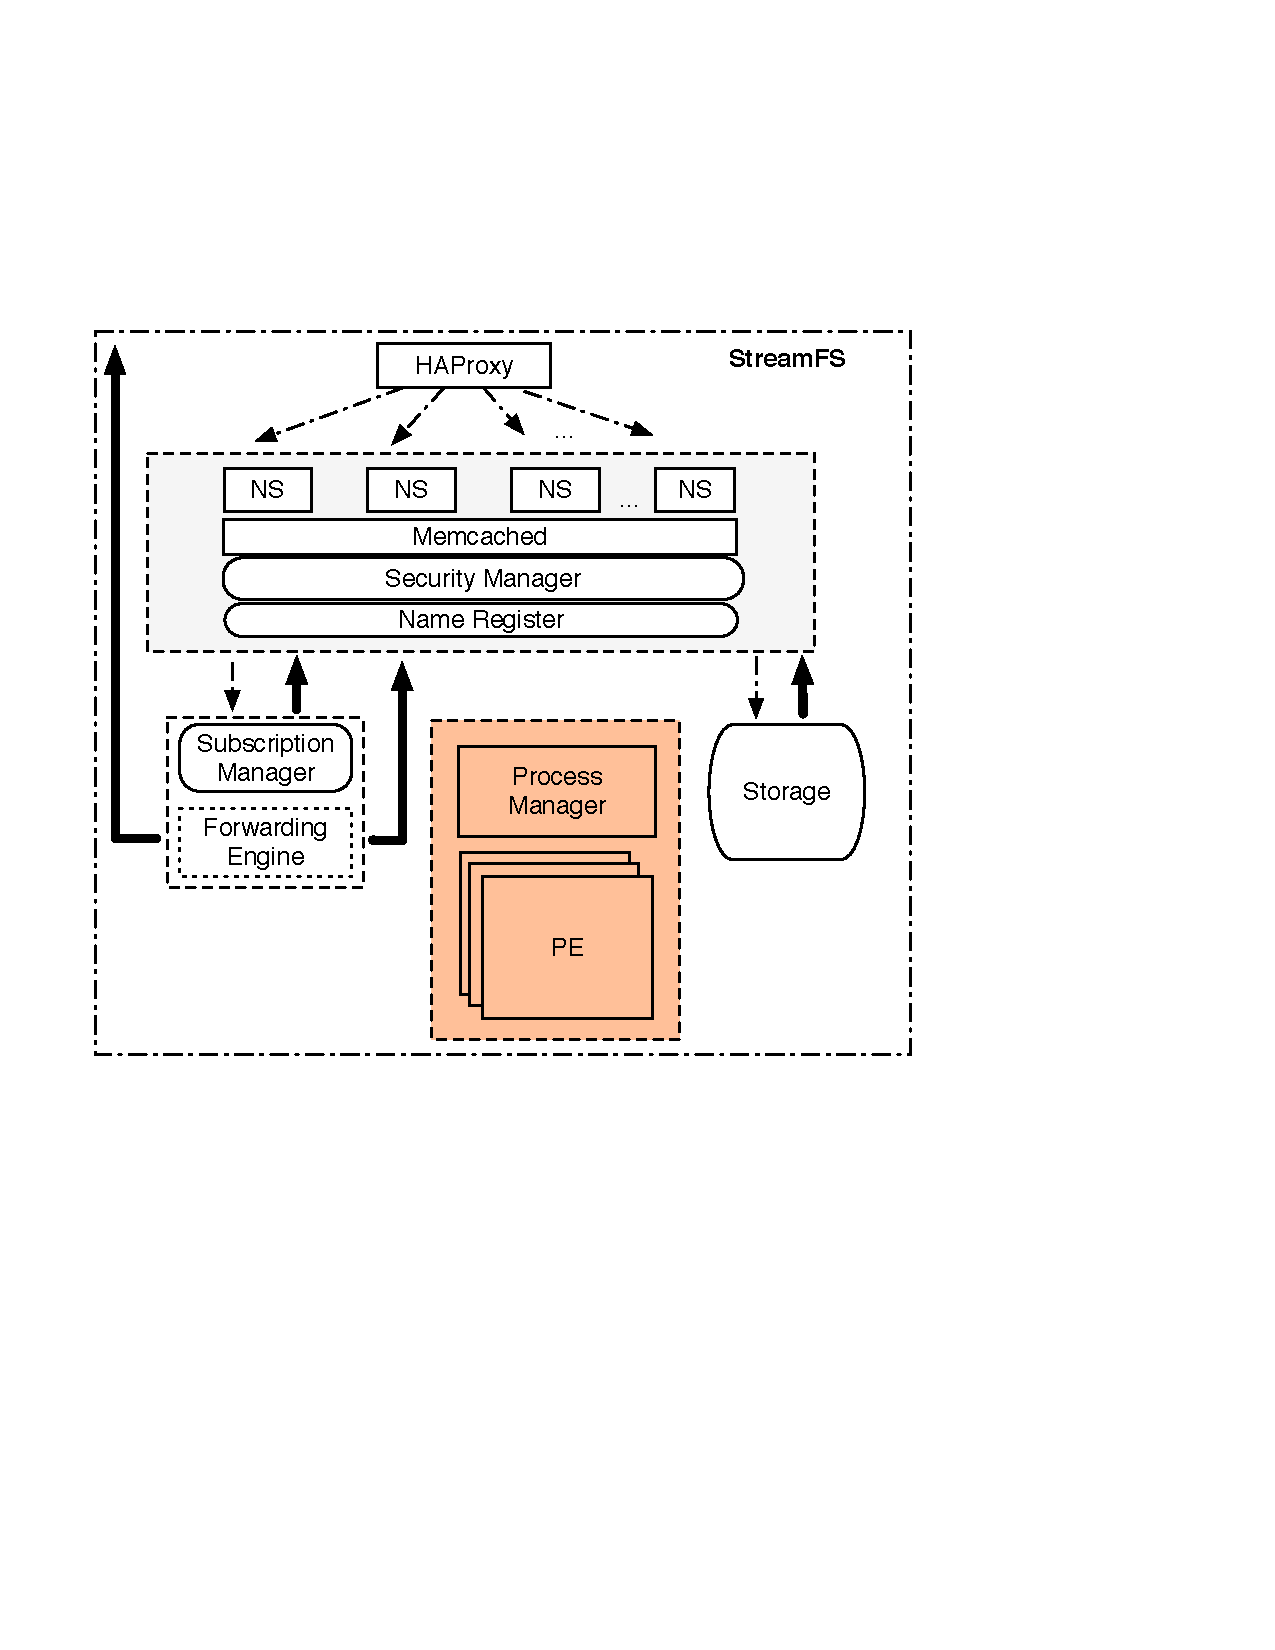
\includegraphics[width=.55\columnwidth]{figs/procmngr}
\caption{The process manager manages a cluster of processing element and connection to external processing units.  It works
closely with the subscription manager to forward data between elements.}
\label{fig:procmngr}
\end{figure}


The process manager works closely with the name register to manage process definition files and process instances.  Process definition files
are those that are submitted to the server by the user, that define a function to run on the streaming data.  Once data is piped to the process
definition file, the process manager spawns and instance of the definition file on one of the process-element (PE) execution servers.  The PE
creates a buffer for incoming data and sets up a job to run periodically according to the specification for the internal processing job.
The internal processing job is mapped to a file that is accessible in StreamFS.  It contains various statistics about the job that is running, such
as the streams that feed it, the last time it ran, the amount of time it took to run, the period of execution, etc.
If the user deletes the file, the process manager contact the corresponding PE server that contains the job and the job is killed.  Once the job
is killed it informs the process manager which informs the name register to remove the file.

For jobs that are more complex and need to run externally, we created an client-stub that runs like a mini-PE.  It spawns a job on the client
side when a user pipes data into it.  It manages all instances of running jobs on the client server and it processes requests associated with
operations on the corresponding instance file represented in StreamFS.  Figure~\ref{fig:procmngr} shows the components of the StreamFS architecture
that handles all processing elements.















